\chapter{Thiết kế giải pháp}
\section{Phương pháp kiểm tra Black Box}
Theo định nghĩa\cite{blackbox}, phương pháp black box còn được biết đến là kiểm tra hành vi, là một phương pháp kiểm thử phần mềm trong đó cấu trúc/thiết kế/hiện thực của đối tượng đang được kiểm tra không được biết đến bởi người kiểm tra.
\begin{center}
	\begin{figure}[!ht]
		\centering
		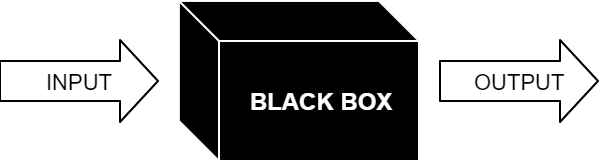
\includegraphics[width=80mm]{images/black-box.png}
		\caption{Phương pháp kiểm tra Black Box}
	\end{figure}
\end{center}
\par
Ứng dụng của chúng tôi sẽ áp dụng phương pháp kiểm tra này để đánh giá SEO cho website mà người dùng nhập vào. Cụ thể, ứng dụng sẽ tìm đến và tải về mã nguồn trang web, sau đó phân tích các thông tin nhận được, so sánh với các tiêu chí mà chúng tôi quy ước sẵn và trả về giao diện hiển thị kết quả cho người dùng.
\par
Với thiết kế này, người dùng sẽ không cần phải có kiến thức về lập trình. Ứng dụng của chúng tôi sẽ thay người dùng làm việc đó. Do đó mang lại trải nghiệm thuận tiện cho người dùng.
\par
Tuy nhiên, với giải pháp này, ứng dụng của chúng tôi sẽ xuất hiện vài khuyết điểm. Do không biết được mã nguồn chính xác của trang web, nên đôi khi trình phân tích mã nguồn của chúng tôi sẽ không ổn định, dẫn đến việc đánh giá sẽ không được chính xác hoàn toàn. Đối với các trang web được sinh ra bằng JavaScript, hiện tại thư viện phân tích mã nguồn của chúng tôi không thể tải về được cú pháp, do đó không thể kiểm tra được những trang web thuộc loại này.
\par
Nhìn chung, với việc áp dụng phương pháp kiểm tra trang web theo cơ chế black box sẽ mang đến trải nghiệm thuận tiện cho người dùng ứng dụng của chúng tôi.
\section{Kịch bản người dùng}
Chúng tôi xây dựng nên kịch bản của ứng dụng dành cho người dùng dựa trên mô hình MTV (Model - Template - View) của Django. Chúng tôi sử dụng sơ đồ bên dưới để trình bày về mô hình ứng dụng của chúng tôi.
\begin{center}
	\begin{figure}[!ht]
		\centering
		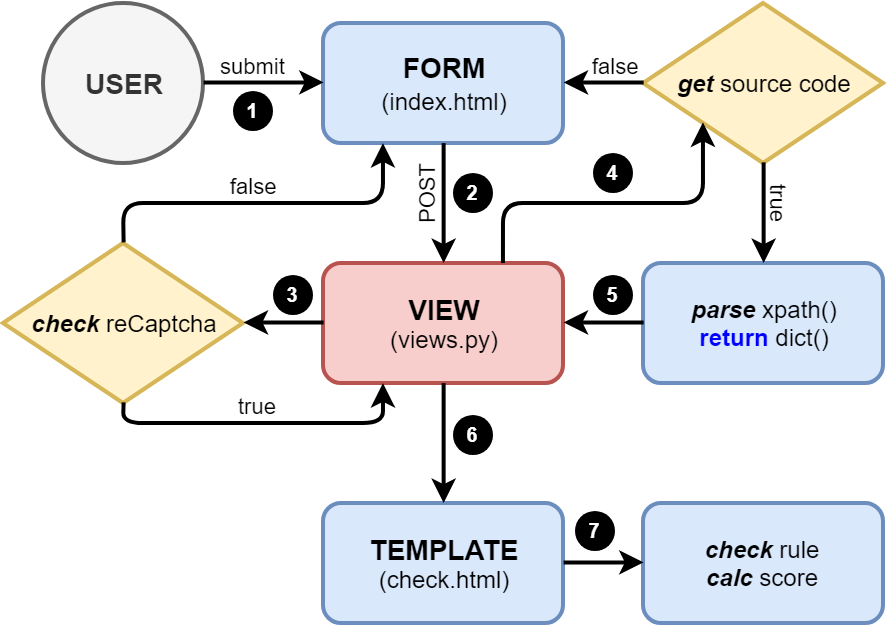
\includegraphics[width=120mm]{images/kich-ban-nguoi-dung.png}
		\caption{Kịch bản người dùng}
	\end{figure}
\end{center}
\begin{enumerate}
	\item Người dùng truy cập vào trang chủ của ứng dụng được lưu ở file \textbf{\texttt{index.html}}, tại đây hiển thị thẻ \textbf{\texttt{input}} để người dùng nhập url website cần kiểm tra.
	\item Khi người dùng bấm vào nút gửi, form sẽ gửi tín hiệu về \textbf{\texttt{VIEW}} với giao thức \textbf{\texttt{POST}}.
	\item Tại đây, chúng tôi có hàm để kiểm tra xem người dùng đã xác thực reCaptcha chưa. Nếu đúng, sẽ đi tiếp đến bước kế tiếp. Ngược lại, chúng tôi sẽ chuyển hướng người dùng về lại trang chủ và thông báo lỗi xác thực reCaptcha.
	\item Khi việc kiểm tra reCaptcha thành công, chúng tôi sẽ tiến hành truy vấn đến liên kết mà người dùng nhập vào, sau đó lấy nội dung source code bằng cách sữ dụng thư viện \textbf{\texttt{requests}}. Tuy nhiên, sẽ có trường hợp liên kết url của người dùng nhập vào bị sai, hoặc vì một lý do nào đó mà thư viện của chúng tôi không thể lấy source code được. Do đó, chúng tôi sử dụng cấu trúc \textbf{\texttt{try/except}} và trả về \textbf{\texttt{false}} nếu liên kết gặp lỗi.
	\item Tại đây, sau khi đã lấy được nội dung source code của trang web, chúng tôi cần định dạng lại bằng thư viện \textbf{\texttt{lxml}} để có thể thực hiện các toán tử \textbf{\texttt{xpath}} phân tích các thành phần trang web từ source code. Chúng tôi khai báo biến \textbf{\texttt{value}} với kiểu dữ liệu là \textbf{\texttt{dict()}} để lưu trữ kết quả sau khi phân tích, với mỗi tiêu chí đánh giá tương ứng với mỗi khóa riêng biệt trong biến \textbf{\texttt{value}}. Sau hàm xử lý này, biến \textbf{\texttt{value}} được trả về để tiếp tục quá trình triển khai trong ứng dụng.
	\item Sau khi nhận được dữ liệu về các yếu tố cần đánh giá, tiếp theo ứng dụng của chúng tôi sẽ truyền những giá trị này sang phía giao diện. Cụ thể, phần giao diện đảm nhiệm xử lý những dữ liệu này nằm ở file \textbf{\texttt{check.html}}.
	\item Với từng giá trị nhận được, chúng tôi sử dụng các thẻ hỗ trợ của Django để tiến hành so sánh với những tiêu chí về đánh giá web. Sau cùng, dựa trên những kết quả so sánh, chúng tôi sẽ sử dụng JavaScript để tính toán điểm số cho trang web dựa trên trọng số và hiển thị lên giao diện người dùng.
\end{enumerate}
\section{Giao diện người dùng}
Chúng tôi sử dụng tính kế thừa giao diện trong Django để thiết kế nên mô hình cho ứng dụng của mình. Ngoài ra, để tạo giao diện đa nền tảng, tối ưu với các thiết bị di động, chúng tôi sử dụng Bootstrap để quản lý tính responsive cho trang web. Bên cạnh đó, chúng tôi sử dụng Font Awesome để hiển thị icon trong trang web.
\par
Trong dụ án của chúng tôi, sẽ có hai phần ứng dụng con.
\begin{itemize}
	\item Checkweb: đây là ứng dụng trọng tâm cho dự án của chúng tôi, nơi chúng tôi xây dựng các hàm kiểm tra và đánh giá SEO cho trang web người dùng cần kiểm tra.
	\item Tips: sẽ là nơi chúng tôi đăng những bài viết về các tiêu chuẩn SEO, ứng dụng này chủ yếu là nhận truy vấn của người dùng và hiển thị giao diện web.
\end{itemize}
\subsubsection{base.html}
Đây là bộ khung cho ứng dụng, được chia thành ba khối cơ bản là \textbf{\texttt{title}} chứa tiêu đề, \textbf{\texttt{content}} chứa nội dung, \textbf{\texttt{script}} chứa các mã JavaScript.
\subsubsection{header.html, footer.html}
Hai file giao diện này có nội dung là hiển thị thanh menu ở đầu trang web và thông tin về dự án ở cuối trang. Thay vì được viết trực tiếp trong file \textbf{\texttt{base.html}}, chúng tôi chia nhỏ từng phần ra để code của chúng tôi được cấu trúc rõ ràng hơn. Sau cùng, chúng được \textbf{\texttt{include}} lại vào file \textbf{\texttt{base.html}} tại vị trí tương ứng cần hiển thị.
\subsubsection{index.html}
File này đóng vai trò là trang chủ trong ứng dụng. Chúng tôi hiển thị một form để người dùng nhập vào URL cần kiểm tra.
\par
Để bảo vệ website chúng tôi tránh liên tục spam truy vấn đến các trang web khác. Chúng tôi sử dụng phương thức POST cho form và sử dụng thêm reCAPTCHA nhằm xác thực người dùng.
\subsubsection{about.html, contact.html}
Hiển thị phần giới thiệu về ứng dụng của chúng tôi đến người dùng và thông tin liên hệ.
\subsubsection{check.html}
Trang này chúng tôi dùng để hiện thị thông tin được phân tích từ website của người dùng nhập vào. Kết quả sẽ được hiển thị bằng thẻ \textbf{\texttt{table}} gồm các cột:
\begin{itemize}
	\item Tiêu chí: Hiển thị các mục mà chúng tôi xem xét trang web người dùng, như là tiêu đề, mô tả và các thẻ khác.
	\item Kết quả: Sử dụng icon từ Font Awesome để cho người dùng biết tiêu chí đó có đạt yêu cầu hay không. Nếu đạt yêu cầu thì sẽ hiển thị icon có dấu tích xanh lá, ngược lại trang web hiển thị dấu x đỏ.
	\item Chi tiết: Mục này chúng tôi dùng để liệt kê ra nội dung được lấy từ trang web của người dùng, ví dụ như nội dung của thẻ tiêu đề, mô tả, hình ảnh\ldots
\end{itemize}
\par
Ngoài ra, chúng tôi sử dụng đoạn JavaScript để tính toán điểm cho website dựa trên kết quả kiểm tra, màu sắc sẽ thay đổi theo từng thang điểm:
\begin{itemize}
	\item $[80, 100]$: Màu xanh lá.
	\item $[50, 80)$: Màu vàng.
	\item $[0, 50)$: Màu đỏ.
\end{itemize}
\par
Nút Trở lại được đặt ở cuối bảng cho phép người dùng quay lại trang chủ để có thể kiểm tra trang web khác.
\section{Bảng đánh giá các tiêu chí SEO}
\begin{table}[!ht]
	\centering
	\begin{tabular}{|c|c|l|}
		\hline
		\textbf{Tiêu chí} & \textbf{Trọng số} & \textbf{Chi tiết}\\
		\hline
		Tiêu đề & 5 & Độ dài lớn hơn 0 và nhỏ hơn 65\\
		\hline
		Mô tả & 5 & Độ dài lớn hơn 0 và nhỏ hơn 160\\
		\hline
		Favicon & 5 & Có ảnh favicon trong trang web\\
		\hline
		Robots & 5 & Có thuộc tính robots trong trang web\\
		\hline
		Thẻ h1 & 5 & Có thẻ h1 trong trang web\\
		\hline
		Thẻ h2 & 3 & Có thẻ h2 trong trang web\\
		\hline
		Robots.txt & 5 & Có file robots.txt trong trang web\\
		\hline
		Sitemap & 5 & Có file sitemap.xml trong trang web\\
		\hline
		Lỗi liên kết & 3 & Không có lỗi liên kết trong trang web\\
		\hline
		CSS nội tuyến & 3 & Không có thuộc tính CSS nội tuyến trong trang web\\
		\hline
		Thuộc tính alt & 3 & Có thuộc tính alt trong hình ảnh\\
		\hline
	\end{tabular}
	\caption{Bảng đánh giá các tiêu chí SEO}
\end{table}